% =========================================================================== %

\begin{frame}[t,plain]
\titlepage
\end{frame}

% =========================================================================== %

\begin{frame}{Scope For Today}
%
\begin{itemize}
\item Slots
	\begin{itemize}
	\item Memory Layout of Classes
	\item Secondary Consequences
	\item Pros and Cons
	\end{itemize}
\item Singletons
	\begin{itemize}
	\item Concept
	\item Realization in Python
	\item Pros and Cons
	\end{itemize}
\item Metaclasses
	\begin{itemize}
	\item Concept
	\item Realization
	\item Use Cases
	\end{itemize}
\end{itemize}
%
\end{frame}

% =========================================================================== %

\begin{frame}{Parking}
%
\begin{center}
	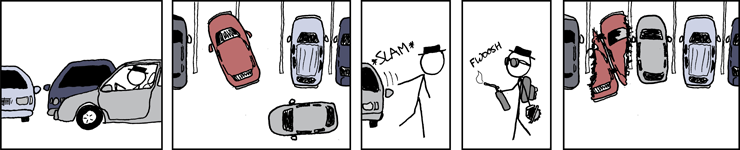
\includegraphics[width=\linewidth]{./gfx/13-xkcd-parking}
\end{center}
%
\begin{center}
	\emph{Police reported three dozen cheerful bystanders,\\yet no one claims to have seen who did it.}

	\vspace{6pt}
	Source: \url{https://xkcd.com/562/}
\end{center}
%
\end{frame}

% =========================================================================== %

\begin{frame}{Recap: Class Instances}
%
\begin{itemize}
\item Attributes are generated dynamically
	\begin{itemize}
	\item Internally, \inPy{class} instances (usually) have a member \inPy{__dict__}\footnote{%
		Keys of \inPy{__dict__} must be \inPy{str}ings. They may, however, contain whitespaces and other non-syntax elements.}
	\item \inPy{instance.new_attribute = value} is (almost) the same as \inPy{instance.__dict__["new_attribute"] = value}
	\item Some extra logic to first check for class attributes
	\item Attribute access actually resolved by \inPy{getattr(instance, attribute)} and \inPy{setattr(instance, attribute, value)}
	\item \inPy{vars(instance)} is same as \inPy{instance.__dict__} 
	\end{itemize}
\item Python's \inPy{class}es are instances of \inPy{type}
	\begin{itemize}
	\item They themselves have their own \inPy{__dict__}
	\end{itemize}
\item[\Thus] Highly modifiable at runtime
\item[\Thus] Noteworthy overhead
\end{itemize}
%
%
\end{frame}

% =========================================================================== %

\begin{frame}[fragile]
%
\begin{codebox}[Approximate C equivalent of a Python object]
\begin{minted}[fontsize=\footnotesize, linenos]{c}
struct_objectInstance {
    // used for garbage collection
    struct objectInstance* _gc_next;    
    struct objectInstance* _gc_prev;
    
    // "Python infrastructure"
    size_t                 refCount;
    struct objectInstance* type;
    
    // contains actual attributes
    struct objectInstance* __dict__;
    // used by weakref module
    struct objectInstance* __weakref__;
};
\end{minted}
\end{codebox}
%
\end{frame}

% =========================================================================== %

\begin{frame}{Problems With This Approach}
%
\begin{itemize}
\item Memory overhead!
	\begin{itemize}
	\item Grows with number of arguments
	\item Typical classes consume 3..5 times more memory than strictly necessary
	\item Overhead scales with number of attributes
	\end{itemize}
\item Source of errors
	\begin{itemize}
	\item Typos at write access silently create new entries in \inPy{__dict__}
	\end{itemize}
\item Solution: \inPy{__slots__} mechanism
	\begin{itemize}
	\item Pack all attributes directly into the \mintinline{c}{struct}
	\item Simply add \inPy{class} attribute \inPy{__slots__ = iterable_of_strings} 
	\item[\Thus] Loose flexibility to add elements at runtime ...
	\item[\Thus] ... unless you explicitly add a \inPy{__dict__} attribute
	\end{itemize}
\item Does not improve lookup speed
	\begin{itemize}
	\item Still some sort of \inPy{dict} lookup, because \inPy{getattr} has to work with slots, too
	\end{itemize}
\end{itemize}
%
\end{frame}

% =========================================================================== %

\begin{frame}[fragile]
%
\begin{codebox}[A Slotted Class]
\begin{minted}[fontsize=\footnotesize, linenos]{python3}
class Foo:
    __slots__ = ("x", "y")
    
    def __init__(self):
        self.x = 1


foo = Foo()

print(foo.x)
# print(foo.y)   AttributeError: 'Foo' object has no attribute 'y'

foo.y = 2
print(foo.y)

# foo.z = 3      AttributeError: 'Foo' object has no attribute 'z'
\end{minted}
\end{codebox}
%
\end{frame}

% =========================================================================== %

\begin{frame}{Side Notes}
%
\begin{itemize}
\item Having a slotted class suppresses the \inPy{__dict__} and \inPy{__weakref__} attributes
	\begin{itemize}
	\item You can still manually add them as slots
	\item \inPy{__slots__ = ("__dict__", ...)}
		\begin{itemize}
		\item Allows dynamically adding attributes
		\item Removes memory overhead of slot-attributes
		\item Removes error check
		\end{itemize}
	\end{itemize}
\item Inheritance
	\begin{itemize}
	\item Slots are inherited
		\begin{itemize}
		\item You get a union of the defined slots in the child class
		\item Redefining slots of parent class is allowed
		\end{itemize}
	\item \inPy{__dict__} and \inPy{__weakref__} are \emph{not} suppressed in child classes (unless the child class has its own \inPy{__slots__} attribute)
	\end{itemize}
\item Getting the memory footprint
	\begin{itemize}
	\item Python provides \texttt{sys.getsizeof(obj)}
	\item Results are misleading here -- does not analyze size of \inPy{__dict__} itself
	\item Use $3^{\text{rd}}$ party library function \texttt{pympler.asizeof} for exact values
	\end{itemize}
\end{itemize}
%
\end{frame}

% =========================================================================== %

\begin{frame}
%
\begin{warnbox}[Mutable Slots]
\begin{itemize}
\item \inPy{__slots__} expects any iterable of \inPy{str}ings (except for \inPy{str}ing itself)
\item Should be a \inPy{tuple} (or better: \inPy{frozenset}) of \inPy{str}ings
\item Can also be a mutable iterable
	\begin{itemize}
	\item Changing the content of \inPy{__slots__} does not alter the memory layout!
	\item Adding values to the iterable will lead to \texttt{AttributeError}s
	\item You can add the new attribute to the \inPy{class}' \inPy{__dict__}, but this attribute then will be read-only
	\end{itemize}
\item[\Thus] Don't change the \inPy{__slots__} 
	\begin{itemize}
	\item Neither add, remove or even only rename objects
	\end{itemize}
\end{itemize}
\end{warnbox}
%
\begin{hintbox}[Don't get confused]
\small
As a class attribute, \inPy{__slots__} is stored in the \inPy{__dict__} of the \inPy{class} object; only in the instance, the \inPy{__dict__} is suppressed.
\end{hintbox}
%
\end{frame}

% =========================================================================== %

\begin{frame}{Pros and Cons of Slotted Classes}
%
\begin{itemize}
\item Pros
	\begin{itemize}
	\item Primary use: Reduce memory overhead
		\begin{itemize}
		\item Usually, memory is not a concern
		\item When you deal with lots of instances, this may be relevant
		\end{itemize}
	\item Avoid spelling errors
	\end{itemize}
\item Cons
	\begin{itemize}
	\item Removes Flexibility
	\item Few people familiar with \inPy{__slots__}
	\item Expected behaviors no longer available
		\begin{itemize}
		\item \inPy{vars(obj)} accesses \inPy{__dict__}, throws error when suppressed
		\end{itemize}
	\item Possibility to have \inPy{__slots__} \emph{and} \inPy{__dict__} exacerbates problems
	\end{itemize}
\end{itemize}
%
\end{frame}

% =========================================================================== %

\begin{frame}[fragile]
%
\begin{codebox}[RPG Game Extract Using Slots]
\begin{minted}[fontsize=\scriptsize, linenos]{python3}
CATEGORIES = ("strength", "charisma", "intelligence", "dexterity")
class Item:
    def __init__(self, name, category, boost):
        self.name = name
        self.category = category
        self.boost = boost

class Person:
    __slots__ = ("name", "backpack", *CATEGORIES)
    
    def __init__(self, name):
        self.name = name
        self.backpack = []        
        for category in CATEGORIES:
            setattr(self, category, random.randint(5, 10))

    def get_property(self, category):
        value = getattr(self,category)
        for item in self.backpack:
            if item.category == category: value += item.boost
        return value
\end{minted}
\end{codebox}
%
\end{frame}

% =========================================================================== %

\begin{frame}{Extrapolating}
%
\begin{center}
	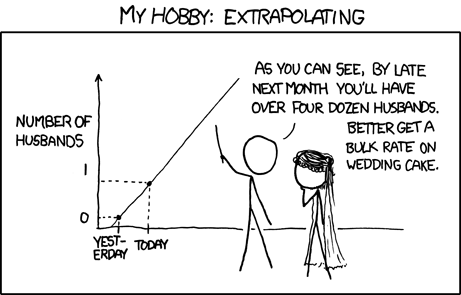
\includegraphics[width=.5\linewidth]{./gfx/13-xkcd-extrapolating}
\end{center}
%
\begin{center}
	\emph{By the third trimester, there will be hundreds of babies inside you.}

	\vspace{6pt}
	Source: \url{https://xkcd.com/605/}
\end{center}
%
\end{frame}

% =========================================================================== %

\begin{frame}{Singletons}
%
\begin{itemize}
\item Idea: \inPy{class} that is guaranteed to ever only have one instance
\item Hijack instantiation process
	\begin{itemize}
	\item Have a \inPy{class} member \texttt{instance} initialized to \inPy{None}
	\item \inPy{if instance is None: self.instance = get_new_instance()}\footnote{%
		We'll see in a minute how this \texttt{get\_new\_instance} could look like}
	\item \inPy{return self.instance}
	\end{itemize}
\item Put this logic in the \emph{true constructor}
	\begin{itemize}
	\item \inPy{__init__} is only initializer, \ie instance already exists when method is called
	\item \inPy{__new__} is true constructor, returns instance
	\end{itemize}
\item But why would we want that?
	\begin{itemize}
	\item Essentially global variable with extra functionality
	\item Example uses: Logging, drivers objects, caching, settings with complex initialization, special constants
	\item Python's \inPy{None} is a Singleton! \Thus This is how \inPy{if variable is None: ...} works
	\end{itemize}
\end{itemize}
%
\end{frame}

% =========================================================================== %

\begin{frame}[fragile]
%
\begin{codebox}[Singleton Blueprint]
\begin{minted}[fontsize=\scriptsize, linenos]{python3}
class Singleton:
    _instance = None
    
    def __new__(cls, *args, **kwargs):
        if not cls._instance:
            cls._instance = super(Singleton, cls).__new__(cls, *args, **kwargs)
        return cls._instance


if __name__ == '__main__':
    s1 = Singleton()
    s2 = Singleton()
    
    if id(s1) == id(s2):
        print("Same")
    else:
        print("Different")
\end{minted}
\end{codebox}
%
\end{frame}

% =========================================================================== %

\begin{frame}{Analyzing the Constructor}
%
\begin{itemize}
\item Signature \inPy{(cls, *args, **kwargs)}
	\begin{itemize}
	\item \inPy{cls} is like \inPy{self}, but refers to the \emph{class} being instantiated
	\item Other arguments: arbitrary, from instantiation itself (\inPy{foo = Foo(args, keyword=kwarg, ...)})
	\end{itemize}
\item Call to \inPy{super(Singleton, cls)}
	\begin{itemize}
	\item Returns a proxy object that behaves like an instance of the parent \inPy{class}(es)
	\item Inheriting from multiple \inPy{class}es requires \emph{MRO} (method resolution order) mechanic
		\begin{itemize}
		\item \inPy{__mro__} is an iterable of \inPy{type}s, exists for each \inPy{type}
		\item Determines in which order to look for methods and attributes
		\item Contains own class and all parent classes
		\end{itemize}
	\item First argument: for whom to find next parent/sibling class
	\item Second argument: whose MRO list to look through
	\end{itemize}
\item Call to \inPy{super(...).__new__(cls, *args, **kwargs)}
	\begin{itemize}
	\item Percolate instantiation request up to \inPy{object}
	\item In the end, \inPy{object} will know whom to instantiate (\inPy{cls}) and thus how much memory to reserve
	\end{itemize}
\end{itemize}
%
\end{frame}

% =========================================================================== %

\begin{frame}[fragile]
%
\begin{columns}[T]
\column{.55\linewidth}
\begin{codebox}[Tangent: Method Resolution Order]
\begin{minted}[fontsize=\scriptsize, linenos]{python3}
class Base:
    def __init__(self, *args, **kwargs):
        pass

class A(Base):
    def __init__(self, *args, **kwargs):
        print("A")
        super(A, self).\
            __init__(*args, **kwargs)

class C(A):
    def __init__(self, arg, *args, **kwargs):
        print ("C","arg=",arg)
        super(C, self).\
            __init__(arg, *args, **kwargs)

...
print("MRO:", [x.__name__ for x in E.__mro__])
E("explicit")
\end{minted}
\end{codebox}
%
\column{.22\linewidth}
\begin{cmdbox}[Output]
\begin{minted}[fontsize=\scriptsize]{text}
MRO: ['E',
      'C',
      'A',
      'D',
      'B',
      'Base',
      'object']

E arg= explicit
C arg= explicit
A
D arg= explicit
B
\end{minted}
\end{cmdbox}
%
\column{.15\linewidth}
\begin{center}
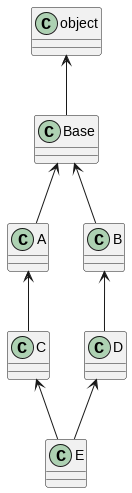
\includegraphics[width=.7\linewidth]{./gfx/13-class-inheritance}
\end{center}
\end{columns}
%
\end{frame}

% =========================================================================== %

\begin{frame}{Notes}
%
\begin{itemize}
\item \texttt{instance = SomeClass(...)} is actually resolved to \inPy{instance = SomeClass.__call__(...)}
	\begin{itemize}
	\item The \inPy{__call__} in turn calls \inPy{__new__} and \inPy{__init__}\footnote{%
		\inPy{__init__} is only called, if the type of the return value of \inPy{__new__} matches the requested type.
		} 
	\item Writing \texttt{Singleton()} repeatedly \emph{does} re-initialize the object
	\item[\Thus] Best to put initialization in the \inPy{if} branch of \inPy{__new__}
	\end{itemize}
\item You cannot meaningfully inherit the Singleton property
	\begin{itemize}
	\item \texttt{instance} is a class attribute of the parent class, shared between \emph{all} children
	\item It is possible to define a singleton decorator or a singleton metaclass (see later)
	\item You don't have to write either of them yourself
		\begin{itemize}
		\item Decorator: \url{https://pypi.org/project/singleton-decorator/}
		\item Metaclass: \url{https://pypi.org/project/python-singleton-metaclasses/}
		\end{itemize}
	\end{itemize}
\end{itemize}
%
\end{frame}

% =========================================================================== %

\begin{frame}{Pros and Cons of Singletons}
%
\begin{itemize}
\item Advantages
	\begin{itemize}
	\item Allows lazy initialization
	\item Open up their own namespace
	\end{itemize}
\item Highly criticized pattern
	\begin{itemize}
	\item Same problem as with global variables
	\item Cause entire code to be coupled, hides dependencies
		\begin{itemize}
		\item State is carried through the entire lifetime of the program
		\item Difficult to test
		\end{itemize}
	\item Violates Single Responsibility Principle
		\begin{itemize}
		\item Control their own life cycle AND their primary task
		\item More responsibilities implies more changes
		\end{itemize}
	\item Violates Open/Closed Principle
		\begin{itemize}
		\item \enquote{Open for extension, closed for modification}
		\item Allow adding code and calling existing routines, but no changes
		\item Deriving from a Singleton not possible \\
			\Thus need to change code when adding functionality
		\end{itemize}
	 \end{itemize} 
\end{itemize}
%
\end{frame}

% =========================================================================== %

\begin{frame}{Tangent: SOLID Principles}
%
\scriptsize The 1994 Book \emph{\color{blue} \href{https://en.wikipedia.org/wiki/Design_Patterns}{Design Patterns}} by the Gang of Four\footnote{%
	\tiny
	The Code Design Gurus Erich Gamma, Richard Helm, Ralph Johnson and John Vlissides.\\
	Not to be confused with \emph{\color{blue} \href{https://en.wikipedia.org/wiki/Gang_of_Four}{The Gang of Four: Maoist faction in the Chinese Communist Party}}
	} postulates these principles your code should satisfy:
%
\begin{itemize}
	\setlength\itemsep{0em}
	\item \textbf{S}ingle Repsonsibility Principle
		\begin{itemize}
		\scriptsize
		\item Each class does one thing and one thing only
		\end{itemize}
	\item \textbf{O}pen/Closed Principle Principle
		\begin{itemize}
		\scriptsize 
		\item Open for extension, closed for change
		\end{itemize}
	\item \textbf{L}iskov Substitution Principle
		\begin{itemize}
		\scriptsize 
		\item A function that expects a base class should operate equally well with a child class
		\end{itemize}
	\item \textbf{I}nterface Segregation Principle (More Java-Specific)
		\begin{itemize}
		\scriptsize 
		\item Clients should not be forced to depend upon interfaces that they do not use.
		\end{itemize}
	\item \textbf{D}ependency Inversion (More Java-Specific)
		\begin{itemize}
		\scriptsize 
		\item High-level modules should not import anything from low-level modules.\\
			Both should depend on abstractions (e.g., interfaces).
		\item Abstractions should not depend on details.\\
			Details (concrete implementations) should depend on abstractions.
		\end{itemize}
\end{itemize}
%
\end{frame}

% =========================================================================== %

\begin{frame}{Consensus: Use Singletons Only In A Very Few Specific Cases}
%
\begin{columns}[T]
\column{.6\linewidth}
\begin{itemize}
\item Logger -- Wrapper around global handle to file
	\begin{itemize}
	\item Methods for formatted printing
	\item Destructor -- flush/close the file
	\end{itemize}
\item Read-only object with complex initialization
	\begin{itemize}
	\item Config object initialized from a file
	\item (In practice still: often modifiable, Settings dialog)
	\end{itemize}
\item Caches
	\begin{itemize}
	\item Store expensive-to-compute elements once they are prepared
	\item Having multiple caches defies the purpose
	\end{itemize}
\end{itemize}
%
\column{.35\linewidth}
\begin{center}
	\href%
		{https://preview.redd.it/singletons-are-bad-v0-fpi02bqw44pa1.jpg?width=640&crop=smart&auto=webp&s=9c976bd4d3fe3715677a0bb86161520539c0ca3d}%
		{
\includegraphics[width=\linewidth]{./gfx/13-singletons-meme}}
\end{center}
\end{columns}
%
\begin{itemize}
\item Device drivers
	\begin{itemize}
	\item Only one instance of software may \enquote{talk} to a device at any given time
	\end{itemize}
\end{itemize}
%
\end{frame}

% =========================================================================== %

\begin{frame}[fragile]
%
\begin{codebox}[Singleton Wrapper by GitHub User \href{https://github.com/Kemaweyan/singleton_decorator/blob/master/singleton_decorator/decorator.py}{Kemaweyan}]
\begin{minted}[fontsize=\scriptsize, linenos]{python3}
class _SingletonWrapper:
    def __init__(self, cls):
        self.__wrapped__ = cls
        self._instance = None

    def __call__(self, *args, **kwargs):
        if self._instance is None:
            self._instance = self.__wrapped__(*args, **kwargs)
        return self._instance

def singleton(cls):
    return _SingletonWrapper(cls)
 
@singleton   
class Solo:
    def do_stuff(self):
	    print("Stuff done by", hex(id(self)))

instance = Solo()
instance.do_stuff()
Solo().do_stuff()
\end{minted}
\end{codebox}
%
\end{frame}

% =========================================================================== %

\begin{frame}{Advanced Technology}
%
\begin{center}
	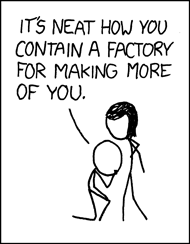
\includegraphics[width=.25\linewidth]{./gfx/13-xkcd-advanced-technology}
\end{center}
%
\begin{center}
	\emph{We are sexy, sexy Von Neumann machines.}

	\vspace{6pt}
	Source: \url{https://xkcd.com/387/}
\end{center}
%
\end{frame}

% =========================================================================== %\\

\begin{frame}{Metaclasses}
%
\begin{itemize}
\item Remember: \inPy{class}es are \inPy{object}s themselves\footnote{%
		We also say, \inPy{class}es are \emph{first class citizens} of Python}
	\begin{itemize}
	\item They can be passed as arguments, may be modified at runtime, ...
	\item They belong to a \inPy{class}, too!
	\item[\Thus] The \inPy{class} of a \inPy{class} is a metaclass
	\end{itemize}
\item What is defining metaclasses good for?
	\begin{itemize}
	\item Mostly changing what happens when you instantiate \inPy{class}es
	\item Designing inheritable meta properties
	\end{itemize}
\end{itemize}
%
\begin{defbox}[Quote]
\footnotesize
\emph{Metaclasses are deeper magic than 99\% of users should ever worry about.
If you wonder whether you need them, you don’t 
(the people who actually need them know with certainty that they need them, and don’t need an explanation about why).}
\begin{flushright}
\color{blue} \href{https://en.wikipedia.org/wiki/Tim_Peters_(software_engineer)}{Tim Peters}
\end{flushright}
\end{defbox}
%
\end{frame}

% =========================================================================== %

\begin{frame}{Defining a \texttt{class} -- Unconventional Alternative Way}
%
\begin{itemize}
\item Keyword \inPy{type}, Usage 1:
	\begin{itemize}
	\item Returns the \inPy{class} of any given object
	\item \inPy{type(some_class) == type}
	\end{itemize}
\item Keyword \inPy{type}, Usage 2: \inPy{type} is a \inPy{class} itself!
	\begin{itemize}
	\item More specifically, a metaclass
	\end{itemize}
\item[\Thus] We can use the Constructor of type \inPy{type} to generate new \inPy{class}es!
	\begin{itemize}
	\item Three arguments: \texttt{name}, \texttt{bases}, \texttt{members}
	\item \texttt{name}: \inPy{str}ing, becomes the new \inPy{class}' \inPy{__class__} attribute
	\item \texttt{bases}: \inPy{tuple}, lists the new \inPy{class}' parent \inPy{class}es
	\item \texttt{members}: \inPy{dict}, becomes the new \inPy{class}' \inPy{__dict__} attribute
	\end{itemize}
\end{itemize}
%
\end{frame}

% =========================================================================== %

\begin{frame}[fragile]
%
\begin{codebox}[A convoluted way of defining classes]
\begin{minted}[fontsize=\scriptsize, linenos]{python3}
A = type('A', (), {'attribute': 0})
# class A:
#     attribute = 0

B = type('The class B', (A,), {})
# class B(A):
#     __class__ = "The class B"

a = A()
b = B()

print(f"{type(A)=}")           # type(A)=<class 'type'>
print(f"{type(a)=}")           # type(a)=<class 'Module.A'>
print(f"{type(B)=}")           # type(B)=<class 'type'>
print(f"{type(b)=}")           # type(b)=<class 'Module.The class B'>
print(f"{b.__class__=}")       # b.__class__=<class 'Module.The class B'>

print(f"{b.attribute=}")       # b.attribute=0
print(f"{isinstance(b, A)=}")  # isinstance(b, A)=True
print(f"{issubclass(B, A)=}")  # issubclass(B, A)=True
\end{minted}
\end{codebox}
%
\end{frame}

% =========================================================================== %

\begin{frame}[fragile]{What We've Got So Far: Defining \inPy{class}es At Runtime}
%
\begin{itemize}
\item All parameters to \inPy{type} are runtime objects
	\begin{itemize}
	\item We can define arbitrary \inPy{class}es at runtime
	\item Even with methods
		\begin{itemize}
		\item Using lambdas:\\
			\inPy{type(..., {"method" : lambda self : print(self.attribute)})}
		\item Using proper functions: \\
			\inPy{def _new(cls, *args, **kwargs): ...} \\
			\inPy{type(..., {"__new__" : _new})}
		\end{itemize}
	\end{itemize}
\item So, if we could redefine \inPy{type}, we imbue some new behaviour on all new classes
	\begin{itemize}
	\item Sadly (gladly), this is forbidden
	\item We cannot \inPy{type.__new__ = _new}
		\begin{itemize}
		\item Affecting \emph{all} classes defined after this is probably a bad idea
		\end{itemize}
	\item But we can inherit from \inPy{type} and set our custom behaviour there
	\end{itemize}
\end{itemize}
%
\end{frame}

% =========================================================================== %

\begin{frame}[fragile]
%
\begin{codebox}[Singleton Metaclass]
\begin{minted}[fontsize=\scriptsize, linenos]{python3}
class SingletonMeta(type):
    def _new(cls, *args, **kwargs):
        if cls._instance is None:
            cls._instance = super(cls, cls).__new__(cls, *args, **kwargs)
        return cls._instance

    def __init__(cls, name, bases, members):
        cls._instance = None
        cls.__new__ = SingletonMeta._new

SomeSingleton = SingletonMeta('SomeSingleton', (), {})
inst_1 = SomeSingleton()
inst_2 = SomeSingleton()
print(inst_1 is inst_2)
\end{minted}
\end{codebox}
%
\end{frame}

% =========================================================================== %

\begin{frame}[fragile]
%
\begin{codebox}[Getting rid of the awkward Class Instantiation]
\begin{minted}[fontsize=\scriptsize, linenos]{python3}
class SingletonMeta(type):
    ...

class SomeSingleton(metaclass = SingletonMeta):
    # business logic here

inst_1 = SomeSingleton()
inst_2 = SomeSingleton()
print(inst_1 is inst_2)
\end{minted}
\end{codebox}
%
\begin{hintbox}[A Convenient Syntax]
\footnotesize
The call

\vspace{3pt}
\inPy{MetaClass(name, bases, members)}
\vspace{3pt}

is built automatically from

\begin{minted}{python3}
class Name (metaclass = MetaClass, bases):
    members
\end{minted}
\end{hintbox}
%
\end{frame}

% =========================================================================== %

\begin{frame}[fragile]{All Is One And One Is All}
%
\begin{codebox}[Instantiating a normal object]
\begin{minted}[fontsize=\scriptsize]{python3}
instance = Class(*args, **kwargs)
    -> Class.__call__(*args, **kwargs)
        -> result = Class.__new__(Class, *args, **kwargs)
        -> result.__init__(*args, **kwargs)
        -> return result
\end{minted}
\end{codebox}
%
\vspace{-3pt}
\begin{codebox}[Defining a new class]
\begin{minted}[fontsize=\scriptsize]{python3}
class Class(metaclass = MetaClass, bases): 
    members

-> Class = MetaClass('Class', bases, members)
    -> MetaClass.__call__('Class', bases, members)
        -> result = MetaClass.__new__('Class', bases, members)
        -> result.__init__('Class', bases, members)
        -> return result
\end{minted}
\end{codebox}
%
\end{frame}

% =========================================================================== %

\begin{frame}{Wassitgudfor}
%
\begin{itemize}
\item Initial Quote by Tim Peters: few things you cannot do with decorators and inheritance
\item Blueprints incompatible with inheritance
	\begin{itemize}
	\item Singletons
	\end{itemize}
\item Registry
	\begin{itemize}
	\item Scenario: Each class belonging to a metaclass should automatically be added to a \inPy{list}
	\item Useful for Unittest frameworks
		\begin{itemize}
		\item Define a number of classes, each of which has a \texttt{run} method
		\item Auto-Register them in \inPy{list testCases}
		\item \inPy{for testCase in testCases: testCase.run()}
		\end{itemize}
	\end{itemize}
\item Immutable Variables
	\begin{itemize}
	\item Redefine \inPy{__setattr__}
	\end{itemize}
\item Overloaded Methods
	\begin{itemize}
	\item See \url{https://www.youtube.com/watch?v=yWzMiaqnpkI}
	\end{itemize}
\end{itemize}
%
\end{frame}

% =========================================================================== %